\section{Searching for WIMPs} \label{Chapter2}

The search for WIMPs can be separated in three categories: indirect detection, WIMP creation, and direction detection experiments.  In this chapter, we will provide a brief overview of the ongoing efforts in each of these fields. Indirect detection experiments search for remnants of WIMP annihilation such as gamma-rays, positrons, and neutrinos using both space based and ground based detectors.  These experiments will be discussed in section~\ref{indi}. In section~\ref{LHCWIMP}, we'll discuss high energy particle colliders such as the LHC, which are used to search for WIMPs in the form of missing energy signals during their particle collisions.   Direct detection experiments, which search for the scattering of dark matter particles on atomic nuclei, will be discussed in section~\ref{direct} and will be the topic of this thesis from Chapter~\ref{LUXChap} onward. 

\subsection{Indirect Detection Experiments}\label{indi}

In section~\ref{WIMPSandSUSY} we discussed the annihilation of CDM particles such as WIMPs during the early universe.  The WIMP annihilation cross section must be close to $\sigma_\nu \sim 3\times 10^{-26}$~cm$^3$/s to account for the observed abundance of dark matter, which provides a well defined target for indirect detection experiments.~\cite{DMCross}  WIMP annihilation may produce any standard model particle that is not kinematically forbidden. Numerous indirect detection experiments search for the gamma-ray, neutrino, and positron annihilation remnants in gravitational wells where the dark matter density is expected to be high, such a the center of the Sun, the center of the Milky Way, or the center of neighboring galaxies.   In the following sections, we will discuss efforts to detect each of these annihilation products separately.

\subsubsection{Gamma-Ray Experiments}

If a WIMP ($\chi$) annihilates directly into a photon ($\gamma$) and another particle ($X$), the photon is mono-energetic with an energy given by
\begin{equation} \label{WIMP-penergy}
E_{\gamma} = m_{\chi} \left(1-\frac{m_X^2}{4m_\chi^2} \right)
\end{equation}
where $m_\chi$ is the mass of the WIMP and $m_X$ is the mass of the remnant particle.~\cite{Fermit-LAT} At the GeV energy scale photons interact with matter via electron-positron pair production, leading to an interaction length much shorter than the thickness of Earth's atmosphere.  As a result, any experiment seeking to directly detect gamma-ray radiation from WIMP annihilation must be based in space.  Satellites such as the Fermi-LAT detect the electron-positron pairs produced by gamma-ray interaction in a detector made of a dense material (in the case of Fermi-LAT, tungsten is used).  These space-based detectors are hindered by the numerous sources of background radiation present in astrophysical data, and are therefore unable to make significant claim of detection without observing a monoenergetic signal across multiple sources.  Typically, gamma-ray detection experiments measure signals originating from dwarf galaxies, as they have relatively little backgrounds and are therefore ideal for searching for dark matter annihilation signals.   As of 2012 the Fermi-LAT has observed no such line features or significant gamma-ray flux in its data~\cite{Fermi-LAT}. 

When gamma-rays interact with the atmosphere they produce a cascade of secondary particles.  These seconday particles produce Cerenkov radiation as they pass through the atmosphere, allowing ground-based telescopes to search for the gamma-ray product of WIMP annihilation indirectly.  Cosmic ray radiation can also induce Cerenkov radiation in the atmosphere, making the it difficult to distinguish gamma-ray sources from the cosmic ray background.  Ground based experiments employ numerical simulations of atmospheric showers and require an excess of directional gamma-rays above the isotropic background induced by cosmic rays to overcome this challenge~\cite{Knapp}.  As with space based experiments, ground based experiments have yet to observe a gamma-ray flux above background in their data~\cite{HESS}.

\subsubsection{Neutrino Experiments}

Neutrinos from WIMP annihilation can interact with ordinary matter via a charge current interaction or a neutral current interaction.  In a charged current interaction, a high energy neutrino transforms into its lepton partner via a process such as inverse beta decay
\begin{equation}
\bar{\nu_e} + p \rightarrow n + e^+ .
\end{equation}
These neutrino interactions are ideal to work with, since the leptons are easy to detect and allow the neutrino to be flavor-tagged.  However, if a neutrino has less energy than the mass of its lepton partner it can not interact via a charge current interaction.  In a neutral current interaction the neutrino remains as a neutrino but deposits energy and momentum onto a target particle.  If the target is light, such as in the electron interaction
\begin{equation}
\bar{\nu_e} + e^- \rightarrow \bar{\nu_e} + e^- ,
\end{equation}
it can be accelerated above the speed of light in the medium and produce Cerenkov radiation.  

Ground based detectors, such as ANTARES and IceCube, search for the neutrinos produced during dark matter annihilation in the Sun, where WIMPs would accumulate due to scattering on protons.  The high energy neutrino signals would present as Cerenkov radiation produced by muon tracks in charged current interactions at the GeV-TeV energy scale, which would in turn be observed by large photo-multiplier arrays buried deep in a transparent medium, such as the antarctic ice.  Such a signal would be a strong indication of dark matter, since no other processes are expected to produce it.  

Unlike direct detection experiments, where the spin-dependent scattering cross section is a function of the  expectation values of the proton and neutron spin operators in the target nucleus, neutrino observation experiments can place strong limits on the spin dependent cross since they are directly measuring annihilation remnants.  Such limits are strongly dependent on assumptions for the dark matter annihilation process, and are therefore more model-dependent than direct detection experiments.  So far, neutrino observation experiments have not observed any dark matter annihilation signal from dark matter particles at the center of the Sun or in nearby galaxy clusters, but have set the world's best spin-dependent cross section limits for WIMPs in the process~\cite{IceCube, IceCube2}.

\subsubsection{Positron Experiments}

Positrons can be produced with a varying spectrum via direct annihilation of dark matter to positron-electron pairs or by annihilations to ZZ or W$^+$W$^-$~\cite{Cheng,Kamionkowsk}.  These positrons do not travel in straight lines from their source due to galactic magnetic fields.  Due to their low mass, electrons and positrons lose energy via inverse Compton scattering and synchrotron radiation as they travel from source to observer. The energy loss increases with the square of the electron energy, such that the power law energy spectrum is steepened at the location of the observer, resulting in an expectation of $\sim$ E$^{-3}$~\cite{PEBS}. 

The inelastic collision of cosmic-ray protons and $\alpha$-particles produce charged pions, which in turn produce secondary positrons and electrons in roughly equal amounts via the $\pi-\mu-e$ decay chain~\cite{Stecker}.  For secondary electrons and positrons, the source spectrum would therefore follow the energy spectrum of ambient protons, which is approximately $\sim$ E$^{-3.7}$ after radiative loss during transit.  If the only source of positrons was from secondary production, and astrophysical sources produced electrons, we would then expect the positron fraction $e^+/(e^+ + e^-)$) to decrease smoothly with energy~\cite{PEBS}. Therefore, experiments which seek to measure a positron signal from dark matter annihilation observe the positron fraction as a function of energy from the entire galactic halo and compare their results to astrophysical models of positron production.

Experiments such as FERMI-LAT, PAMELA, and AMS-02 have confirmed a rise in the positron fraction at high energy~\cite{FermiPositron,PamelaPositron,AMSPositron}. However, a very high cross section and leptophilic models are required for these observations to be attributed to dark matter annihilation.  Alternative explanations such as local pulsar sources and acceleration of secondary positrons have also been proposed~\cite{Serpico}.



\subsection{WIMP creation in Colliders}\label{LHCWIMP}

Experiments such as ATLAS and CMS are using the Large Hadron Collider (LHC) beneath France and Switzerland to search for the production of WIMPs in high energy particle collisions.  The LHC is a proton-proton collider which should have a large production cross section for colored super symmetric particles.  The WIMP pair production interaction $pp (p\bar{p}) \rightarrow \chi \bar{\chi}$ is of no use in these experiments, since it leaves no observable signal in the detector.  Instead, these experiments try to observe the higher order $pp  \rightarrow \chi \bar{\chi} + jets$ interaction, with the jets serving as a trigger that an event took place.  The dominant background when looking for such an event comes from the electroweak processes where the Z decays into a pair of neutrinos $pp (p\bar{p}) \rightarrow \nu \bar{\nu} + jets$ or the $W^{\pm}$ decays into a neutrino and a lepton $pp (p\bar{p}) \rightarrow l^{-}\bar{\nu} + jets$ or $pp (p\bar{p}) \rightarrow l^{+}\nu + jets$. In a WIMP $+$ jets event the WIMP will exit the detector unseen, producing a signature with missing transverse momentum.  The magnitude of this missing momentum is typically denoted as $E_T^{miss}$.  A model-independent approach shows that $E_T^{miss}$ should be detectable at the LHC under the assumption that all new particles mediating the interaction of WIMPs and standard model particles are too heavy to be produced directly~\cite{Beltran}. However, no excess of events beyond the standard model processes has been observed at the LHC as of yet~\cite{ATLAS}.


\subsection{Direct Detection Experiments}\label{direct}
If dark matter interacts through the weak force then it should be possible to observe WIMPs via nuclear recoils in direct detection experiments. During these events a WIMP will scatter off of a target nucleus in the detector, producing a nuclear recoil signal in the range of 1-100 keV~\cite{Lewin}.   Direct detection experiments typically observe ionization, scintillation, or low temperature phonons produced during the event (or a combination of the three), although some experiments have developed a method of detection based on producing bubbles in a superheated fluid at the site of a recoil.  These signals are susceptible to both nuclear recoil and electron recoil backgrounds so detailed in situ calibrations are required to characterize the detector's response to each type of event.  In this section, we will review the canonical galactic halo model and derive an expression for the WIMP recoil spectrum before discussing different types of direct detection experiments in detail.  The following chapter we will be devoted to one particular direct detection experiment, the LUX detector.

\subsubsection{The Canonical Halo Model}

The canonical halo model treats dark matter as an isothermal spherical distribution that behaves as a non-interacting ideal gas.  The spherical shape of the distribution implies no rotational movement in the bulk of the distribution, otherwise it would flatten into a disk.  The velocity of a WIMP relative to the galactic center, $v_0$, can be approximated by the orbital velocity at a given radius from the galactic center. At the location of the sun, $r \approx 8.5 $ kpc, and $v_0 \approx 220$ km/s~\cite{Piffl}.

The local number density of WIMPs is given by
\begin{equation}
n_\chi = \frac{\rho_\chi}{M_\chi}
\end{equation}
where $\rho_\chi$ is the density of WIMPs in the local vicinity, and $M_\chi$ is the mass of a WIMP particle. The local density of the dark matter halo is estimated to be 0.3 $< \rho_\chi <$ 0.7 GeV/cm$^{3}$~\cite{Gates}.  Assuming the value of $\rho_{\chi} = 0.4$ GeV/cm$^{3}$ from reference~\cite{Lewin} we see that $n_\chi = 0.004 $ per cm$^3$ for a WIMP mass of 100 GeV.  With an average WIMP velocity of $v_0=220$ km/s, this is equivalent to a flux of $\phi_\chi \approx 10^7 M_\chi $~s$^{-1}$cm$^{-2}$, or roughly half a billion WIMPs of $M_\chi = 100$ GeV passing through your hand every second.


\subsubsection{The WIMP Recoil Spectrum}

Lewin and Smith provide a standard derivation of the expected WIMP recoil spectrum in reference~\cite{Lewin}.  Their derivation begins with the differential particle density given by 
\begin{equation}
dn=\frac{n_0}{k} f(\mathbf{v},\mathbf{v_E}) d^3\mathbf{v}
\end{equation}
where $n_0$ is the mean dark matter particle density, $\mathbf{v}$ is the velocity of the WIMP relative to the target, $\mathbf{v_E}$ is the velocity of the earth relative to the WIMP, $f(\mathbf{v},\mathbf{v_E})$ is the WIMP velocity distribution function.  The normalization constant $k$ is given by
\begin{equation}
k=\int_0^{2\pi}\int_{-1}^{1} \int_0^{v_{esc}}  f(\mathbf{v},\mathbf{v_E}) v^2 d(cos\theta)dv
\end{equation}
where $v_{esc}$ is the local escape velocity, so that 
\begin{equation}
\int_0^{v_esc}dn \equiv n_0.
\end{equation}

Note that an annual modulation is induced in the velocity of the earth relative to the dark matter particles, and subsequently induced in the event rate of WIMPs in terrestrial detectors as well, due to the velocity of earth around the sun.  This modulation is given by 
\begin{equation}
v_E = v_0 + 15\cos \left(2\pi \frac{T - 152.5}{365.25} \right)
\end{equation}
where $T$ is measured in days from June 2nd, and $v_0 \approx 220$ km/s is the velocity of the sun around the galactic center. The DAMA/Libra collaboration has claimed a detection a dark matter signal with annual modulation with 9.3 $\sigma$ significance~\cite{Bernabei:2013xsa}.  However, many dark matter experiments have since ruled this result out, so it is likely due some other unidentified modulating phenomenon in the data.
%R. Bernabei et al.  Final model independent result of DAMA/LIBRA-phase1. European Physical Journal C, 73:2648, 2013. doi:10.1140/epjc/s10052-013-2648-7.

We treat the dark matter as a non-interacting ideal gas so that we can assume a Maxwellian dark matter velocity distribution given by
\begin{equation}
f(\mathbf{v},\mathbf{v_E})=e^{(-v+v_{E})^2/v_0^2}.
\end{equation}
Then for $v_{esc}=\infty$ we define
\begin{equation} \label{k-not}
k_0 \equiv (\pi v_0^2)^{3/2},
\end{equation}
and for finite escape velocity $v_{esc}=|\mathbf{v}+\mathbf{v_E}|$,
\begin{equation}
k=k_0 \left[\mbox{erf}(\frac{v_{esc}}{v_0}) - \frac{2}{\sqrt{\pi}} \frac{v_{esc}}{v_0} e^{-v_{esc}^2/v_0^2} \right].
\end{equation}

The event rate per unit mass on a target of atomic mass $A$ (AMU), with cross-section per nucleus $\sigma$ is given by
\begin{equation}
dR=\frac{N_0}{A} \sigma v dn
\end{equation}
where $N_0$ is Avogadro's number ($6.02\times10^{23} $~mol$^{-1}$).  For constant cross section $\sigma=\sigma_0$, the event rate per unit mass is then
\begin{equation}
R=\frac{N_0}{A}\sigma_0 \int v dn \equiv \frac{N_0}{A}\sigma_0n_0\left\langle v\right\rangle .
\end{equation}
Substituting $n_0=\rho_{\chi} / M_{\chi}$ (where $\rho_{\chi}$ and $M_{\chi}$ are the WIMP density and mass, respectively) we define the event rate per unit mass for $v_E=0$ and $v_{esc}=\infty$ as
\begin{equation} \label{R-not}
R_0=\frac{2 N_0 \rho_{\chi}}{\sqrt{\pi} A M_{\chi}} \sigma_0 v_0 = \frac{2 \rho_{\chi} }{\sqrt{\pi} M_{\chi} M_T} \sigma_0 v_0
\end{equation}
where $M_\chi$ is the mass of the WIMP and $M_T$ is the mass of the target, such that 
\begin{equation} \label{intR}
R=R_0 \frac{\sqrt{\pi} \left \langle v \right \rangle}{2 v_0} = R_0 \frac{k_0}{2 \pi v_0^4 k} \int v f(\mathbf{v},\mathbf{v_E}) d^3v.
\end{equation}
In differential form equation~\ref{intR} becomes
\begin{equation} \label{diffR}
dR = R_0 \frac{k_0}{2 \pi v_0^4 k} v f(\mathbf{v},\mathbf{v_E}) d^3v.
\end{equation}

The recoil energy (as measured in the lab frame) of a nucleus struck by a WIMP of kinetic energy $E=\frac{1}{2} M_\chi v^2$ and scattered at an angle $\theta$ in a center-of-mass frame is given by
\begin{equation}
E_R= \frac{1}{2} M_\chi v^2 \frac{2 M_\chi M_T}{(M_\chi + M_T)^2} (1-\cos\theta).
\end{equation}
For isotropic scattering recoils are uniformly distributed over a range of $0 \leq E_R \leq \frac{1}{2} M_\chi v^2 \frac{4 M_\chi M_T}{(M\chi + M_T)^2}$ so
\begin{equation} \label{dRdER}
\frac{dR}{dE_R} = \int_{E_{min}}^{E_{max}} \frac{(M_\chi + M_T)^2}{4 M_\chi M_T E} dR(E)
\end{equation}
where $E_{max} = \frac{1}{2} M_\chi v^2 \frac{4 M_\chi M_T}{(M_\chi + M_T)^2}$ and $E_{min}$ is the smallest WIMP energy which can produce a recoil of energy $E_R$.  Since $E=\frac{1}{2}M_\chi v^2$ and $E_0=\frac{1}{2}M_\chi v_0^2$, $E=E_0 \frac{v^2}{v_0^2}$ and equation~\ref{dRdER} becomes
\begin{equation}
\frac{dR}{dE_R} = \frac{(M_\chi + M_T)^2}{4 M_\chi M_T E_0} \int_{v_{min}}^{v_{max}} \frac{v_0^2}{v^2} dR(v)
\end{equation}
where $v_{min}$ and $v_{max}$ is the WIMP velocities corresponding to $E_{min}$ and $E_{max}$.
Therefore, using equations~\ref{k-not},~\ref{R-not}, and~\ref{diffR} the expected energy recoil spectrum of WIMPs scattering off of a target nucleus is given by
\begin{align} \label{final_dRdER}
\frac{dR}{dE_R} \begin{aligned} = \end{aligned} \frac{(M_\chi + M_T)^2}{4 M_\chi M_T} \frac{k_0 R_0}{2\pi E_0 k v_0^2}  \int_{v_{min}}^{v_{max}} \frac{f(\mathbf{v},\mathbf{v_E})}{v} d^3v \nonumber \\
\begin{aligned} = \end{aligned} \frac{ (M_\chi + M_T)^2}{2M_\chi^2M_T^2} \frac{\rho_\chi}{M_\chi} \frac{\sigma_0}{k} \int_{v_{min}}^{v_{max}} \frac{f(\mathbf{v},\mathbf{v_E})}{v} d^3v
\end{align}
It is conventional to express $\sigma_0$ as the product of $\sigma_0$ at the coherent scattering limit in which the WIMP interacts with the entire nucleus (with momentum transfer $q=0$) and a nuclear form factor $F$ which accounts for the loss of coherence with higher momentum transfer.  Therefore, using the WIMP-nucleus reduced mass given by $\mu\equiv \frac{M_\chi M_T}{M_\chi + M_T}$ equation~\ref{final_dRdER} becomes
\begin{equation} \label{final_dRdER_2}
\frac{dR}{dE_R}=\frac{\sigma_0 \rho_\chi}{2 \mu^2 M_\chi k} F^2(q)  \int_{v_{min}}^{v_{max}} \frac{f(\mathbf{v},\mathbf{v_E})}{v} d^3v, 
\end{equation}
where, as a reminder, $\rho_\chi$ is the local WIMP density, $f(\mathbf{v},\mathbf{v_E})$ is the velocity distribution of WIMPs in the halo, $v_{min}$ is the minimum WIMP velocity able to generate a recoil of energy $E_R$, $v_{esc}$ is the escape velocity for WIMPs in the halo, $\sigma_0$ is the WIMP-nucleus interaction cross sections, and $F(q)$ is the nuclear form factor describing the scattering amplitude for momentum transfer $q$.

The WIMP-nucleus cross section can have both spin-independent (SI) and spin-dependent (SD) components~\cite{Shan}. The SI interaction cross section is given by
\[\sigma_0^{SI}=\frac{4}{\pi}\mu^2 \left[Z f_p + (A - Z) f_n \right]^2,\]
where Z is the atomic number of the target nucleus (the number of protons), A is the atomic mass number of the target nucleus ($A-Z$ is therefore the number of neutrons in the nucleus), and $f_p$ and $f_n$ are the effective scalar couplings of WIMPs to protons and neutrons, respectively.  In this process we must sum over the interactions in each nucleon prior to squaring, since the DeBroglie wavelength associated with the momentum transfer is comparable to, or larger than, the size of the target nuclei, giving rise to a coherence effect across the nucleons.  If the scalar couplings of WIMPs with neutrons and protons are approximately equal (which is the case with the LSP of SUSY), then the SI cross section can be simplified to
\[\sigma_0^{SI} \simeq \frac{4}{\pi}\mu^2 A^2 |f_p|^2. \]
The cross section for SD interactions is given by
\[\sigma_0^{SD}=\frac{32}{\pi}G_F^2\mu^2\frac{J+1}{J} \left[\langle S_p \rangle a_p + \langle S_n \rangle a_n \right]^2, \]
where $G_F$ is the Fermi constant, $J$ is the total spin of the target nucleus, $\langle S_{(p,n)} \rangle$ are the expectation values of the proton and neutron group spins, and $a_{(p,n)}$ are the effective SD WIMP couplings on protons and neutrons.  In SD WIMP-nucleus interactions it is assumed that only unpaired nucleons contribute significantly to the total cross section, since the spins of the nucleons in a nucleus are anti-aligned.  In most cases, the spin independent, coherent term dominates the total WIMP-nucleus cross section due to its $A^2$ dependence on the atomic mass number of the target nucleus.  

A calculation of both the differential and integrated WIMP event rates in single isotope targets of  $^{131}$Xe, $^{73}$Ge, and $^{40}$Ar using a WIMP mass of 100 GeV is included in Figure 4.

\begin{center}
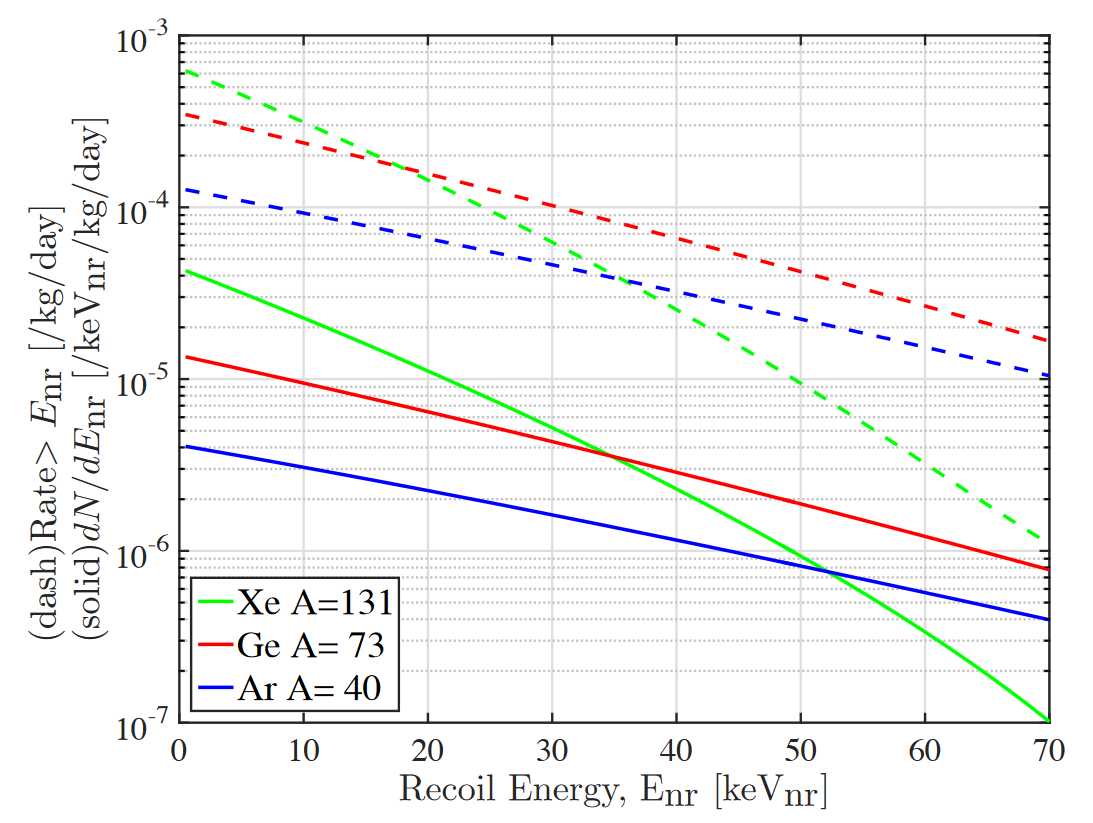
\includegraphics[scale=0.5]{Recoil-spectrum.png}
\captionof{figure}{Calculated differential spectrum in evts/keV/kg/d (solid lines) and the integrated event rate in evts/kg/d (dashed lines)  for $^{131}$Xe, $^{73}$Ge, and $^{40}$Ar assuming a 100 GeV WIMP with spin-indepdent cross section for a WIMP-nucleon of $\sigma=9 \times 10^{-46}$~cm$^2$~\cite{VerbusThesis}.}  
\end{center}

Lighter target nuclei will produce lower event rates in a WIMP detector due to their lower cross sections (resulting from lower $A^2$ contribution in the coherent SI term) and less effective transfer of energy during nuclear recoil events from heavy WIMPs. While heavier target nuclei produce stronger interaction cross sections, they also result in reduced event rates at high energies due to a loss of coherence from form factor suppression. This loss of coherence is not enough to make light target nuclei more ideal than heavy target nuclei at high energies, but the event rate is not enhanced by as much as a naive $A^2$ scaling would suggest.  To maximize efficiency a xenon detector with a low analysis threshold is ideal.

%How discrimination is done in cryogenic experiements (CDMS)
%How its done in bubble chambers
%How its done in liquid noble gas
%single phase (pulse shape, with NR producing singlets instead 						of triplet excimers)
%dual phase (NR has higher charge density, so more 							recombination, so lower S2/S1)

\subsubsection{Backgrounds in Direct Detection Experiments} \label{Backgrounds}

%3.4-25 keVnr = 0.9-5.3 keVee over the same S1 range in LUX
Direct detection experiments search for an extremely rare nuclear recoil signal between 1-100 keV.  These detectors have a number of internal and external backgrounds which could obscure with the WIMP signal.  Therefore, limiting sources of background is critical to maintaining a high discovery potential.  

%Reference Paulo's thesis in here somewhere?
Internal backgrounds can be introduced by radioactive materials present in individual detector components.  Naturally occurring radioisotopes such as $^{232}$Th, $^{238}$U, and $^{40}$K can produce high energy gamma rays which penetrate deep into a detector.  In the case of $^{232}$Th, the decay chain produces high energy gamma rays from radioactive daughters such as $^{228}$Ac, $^{212}$Pb, $^{212}$Bi, and $^{208}$Tl before reaching stable $^{208}$Pb.  Likewise, the $^{238}$U decay chain produce high energy gamma rays from $^{234}$Th, $^{234}$Pa, $^{214}$Pb, $^{214}$Bi before reaching stable $^{206}$Pb.  In the case of $^{40}$K, a 1460.85 keV gamma ray is produced via electron capture decay to $^{40}$Ar.  

In addition to the naturally occurring radioisotopes, cosmogenically activated radioisotopes can also be present inside detector components.  Neutron activation of copper can produce $^{60}$Co, which produces 1.173 MeV and 1.33 MeV gamma rays when it beta decays into $^{60}$Ni with a half life of 5.2714 years.  Neutron activation of titanium produces $^{46}$Sc, which emits 889 keV and 1.12 MeV gamma rays when it beta decays into $^{46}$Ti via electron emission with a half life of 84 days. 

Radon in the detector introduces the $^{222}$Rn and $^{220}$Rn decay chains as additional backgrounds. While most of the daughters in the radon decay chains produce easily vetoed alpha particles, the $^{222}$Rn decay chain includes beta and gamma emitters such as $^{214}$Pb and $^{214}$Bi.  $^{214}$Pb decays into $^{214}$Bi with a half life of 26.8 minutes via beta emission at 1024 keV, and the subsequent $^{214}$Bi decays in $^{214}$Po with a half life of 19.9 minutes via beta emission at 3272 keV.  The $^{220}$Rn decay chain includes $^{212}$Pb, which decays into $^{212}$Bi with a half life of 10.64 hours via beta emission at 573.8 keV.  The $^{212}$Bi then decays via alpha decay into $^{208}$Tl, which can subsequently decay via beta emission.  These beta decays either produce no gamma ray particles (referred to as "naked" beta decays) or high energy gamma rays that can leave the detector without scattering (refereed to as "semi-naked" beta decays), resulting in a background which can not be reduced via detection of a high energy gamma-ray component.  Internal backgrounds from detector components are mitigated with careful screening of the materials which go into a detector; with simulations being used to predict background events arising from materials which make it through the screening process~\cite{PauloThesis}.
	 	
%LUX Ar39 restraints: Need <1 ppb (g/g) in LUX Xe to be comparable to the $10^{-3}$ events per keV/kg/day background estimate
%LUX Kr85 restraints: Need <20 ppt (g/g) in LUX Xe to be comparable to the $10^{-3}$ events per keV/kg/day background estimate		 
Long-lived intrinsic radioisotopes can be present in the detection medium as well.  Cosmogenically activated $^{127}$Xe beta decays via electron capture to $^{127}$I with a half life of 36.358 days.  The captured electron has an 85\% chance of coming from the K shell with an x-ray of 33 keV, a 12\% chance of coming from the L shell with an x-ray of 5.2 keV, and a 3\% chance of coming from higher shells with x-rays of $<$1.2 keV. The subsequent $^{127}$I daughter can decay to ground state via high energy gamma emission, with the gamma frequently leaving the detector without scattering. The $^{127}$Xe activity decays away quickly, so this background can be mitigated by moving the detector underground prior to data collection. $^{39}$Ar is generated by cosmic ray interactions with $^{40}$Ar in a (n,2n) process in the atmosphere and can find its way into a detector's medium.  The 565 keV electron emission decay has a half life of 269 years, placing strong constraints on the amount of $^{39}$Ar that can be present in a detector's medium when data is collected. $^{85}$Kr is produced by man-made processes, such as nuclear fuel re-processing.  As with $^{39}$Ar, the $^{85}$Kr can make its way into a detector's medium where it will beta decay to $^{85}$Rb with a half life of 10.756 years at 687 keV.  These long lived radioisotopes which originate from the atmosphere must be purified from the detector medium prior to data collection to reduce background levels in the detector~\cite{PauloThesis}.

Neutrons are particularly dangerous source of background which can mimic the single scatter nuclear recoil present in a WIMP signal.  While neutrons can be stopped by a few tens-of-meter water-equivalent shielding, cosmic ray muons can penetrate many kilometers of shielding.  Muon interactions in the laboratory can produce "cosmogenic" neutrons at the GeV scale with mean free path much longer than most detectors.  These neutrons can be attenuated by rock or shielding and produce keV scale recoils in WIMP detectors.   Such events are mitigated by tagging the initial muon with a muon veto system, placing external shielding around the detector, and by placing the detector deep underground to limit the muon flux.  Neutrons can also be generated internally via ($\alpha$,n) interactions in construction materials, such as the ($\alpha$ + $^{19}$F $\rightarrow$ $^{22}$Na + n) reaction in fluorine present in PTFE, and from spontaneous fission of $^{238}$U and $^{232}$Th.  

The background mitigation techniques discussed in this section can not completely remove backgrounds from a detector.  To separate any remaining backgrounds from a WIMP signal, detectors use a technique called nuclear recoil discrimination.  Nuclear recoil discrimination does not reduce the total number of background events, but instead seeks to distinguish electron recoil interactions from nuclear recoil interactions and reject the former population.  In the next section we discuss a variety of WIMP detection methods, with each of these methods having its own form of nuclear recoil discrimination. 

%Use http://arxiv.org/pdf/1301.0441v1.pdf as a source
\subsubsection{Direct Detection Methods} 
%Get Sources from bradley thesis http://teacher.pas.rochester.edu:8080/wiki/pub/Lux/LuxRequiredReading/AWB_PhDThesis_20140120.pdf
Ionizing radiation deposits energy in a detector in the form of scintillation light, ionization, and heat.  A variety of WIMP detectors have been constructed that each detect one or two of these channels.  Scintillation detectors use scintillating crystals or liquid scintillators as a target medium. For instance, the DAMA/LIBRA experiment at the Gran Sasso Laboratory in Italy uses room temperature, thallium doped sodium iodide (NaI(Tl)) scintillating crystals as a target medium.  Each crystal is paired with two photomultiplier tubes (PMT) which collect scintillation light from within each crystal.  Annual modulation of the WIMP signal due to the motion of the earth around the sun is used to discriminated background events from WIMP events.  The XMASS detector uses liquid xenon as a target medium.  The scintillation produced in the xenon by recoil events is collected by PMT arrays. Background events from gamma ray sources are attenuated by the liquid xenon's large atomic number (Z=54) and high density, leading to a low background fiducial volume.  This discrimination technique is referred to as "self shielding." 

Single phase liquid argon experiments, such as DEAP and CLEAN, can not take advantage of self shield techniques due to the intrinsic background from $^{39}$Ar.  Instead, these experiments use a technique called pulse shape discrimination to differentiate signal events from background.  Scintillation in liquid noble gases is produced by the decay of singlet or triplet excimers.  The triplet state emits light over a longer period of time, and the light can be suppressed by destructive interactions such as Penning ionization and electron-triplet spin exchange.  Nuclear recoils produce higher excitation densities, and therefore more destructive interactions with the triplet excimers, leading to a difference in the pulse shape of nuclear recoil and electron recoil events. 

Single phase ionization detectors have also been used in the search for dark matter.  The CoGeNT detector in the Soudan Underground Laboratory in Minnesota uses a low input capacitance p-type point contact (PPC) germanium crystal to detect ionization from WIMP interactions.  The detector has energy thresholds as low as 500 eV, allowing the collaboration to search for low mass ($\sim$5 GeV/c$^2$) WIMP particles.  Electron recoil background events scatter at multiple events sites in the germanium crystal, while WIMPs scatter at most once. This leads to a longer rise time in pulses from background events which can be used as another form of pulse shape discrimination.

Phonon detectors are the final type of single signal detectors.  These type of detectors, such as the Cryogenic Underground Observatory for Rare Events (CUORE) in the Gran Sasso National Laboratory, use low heat capacity crystals as a target medium. In the case of CUORE, tellurium dioxide crystals (TeO$_2$) are held at 10 mK to reduce thermal noise.  The low heat capacity of the crystals allows particle interactions to raise the temperature of the crystals, which in turn changes the resistance of neutron transmutation doped germanium thermistors which are glued to the top of each crystal.  A constant current is applied to the thermistors, and the voltage across each thermistor is used as a detection method.  These types of detectors do not have any means of event discrimination, so they rely heavily on the use of radiopure construction materials and background modeling.

In addition to the single signal detectors, many detectors collect data from two of the three energy deposition channels.  The Cryogenic Dark Matter Search (CDMS)  in the Soudan mine records signals from both phonons and ionization.  The detector uses Ge and Si detectors cooled to $\sim$40~mK as a target medium.  The low temperature is required to reduce thermal noise in the detector and to reduce the heat capacity of the target so that the temperature signal is large.  Ionized electrons are drifted to the top of the crystals by an electric field where they are read out using field effect transistors, and the corresponding phonon signal is collected by superconducting transition edge sensors coupled with SQUIDs on the opposite face of each crystal.  The ionization yield of a nuclear recoil is lower than an electron recoil, so the ratio of the two signals is used for nuclear recoil discrimination.

The Cryogenic Rare Event Search with Superconducting Thermometers (CRESST) is a phonon and scintillation detector in the Gran Sasso National Laboratory.  CRESST uses calcium tungstate (CaWO$_4$) crystals, which are cooled to 10 mK to lower thermal noise, as a target medium. As with CDMS, transition edge sensors are used to detect phonons originating from particle interactions in the crystals.  Scintillation light in the crystals absorbed by a silicon light absorber that converts the scintillation photons to heat, which are then detected by secondary thermometers.  A nuclear recoil produces 10-40 times less scintillation light in the CaWO$_4$ crystals than an electron recoil does, so the ratio of the phonon and scintillation signal can be used for nuclear recoil discrimination.

The final class of detectors records the scintillation and ionization signals from particle interactions.  These detectors, which are known as dual phase time projection chambers, use liquid noble scintillators (typically xenon or argon) as a target medium. Primary scintillation light is collected by PMT arrays at the top and bottom of the detector. An electric field is used to drift charge from ionized particles to the top of the detector, where the charge produces a secondary source of scintillation light as it accelerates through the gaseous xenon above the liquid.  The ratio of the primary and secondary scintillation light can be used for nuclear recoil discrimination.  Currently, the most sensitive dark matter detector in the world is a dual phase TPC placed in the Sanford Underground Research Facility in South Dakota.  This detector, known as the Large Underground Xenon detector (LUX), will be discussed in depth in Chapter~\ref{LUXChap}.
